\documentclass{article}

\usepackage[T1]{fontenc}
\usepackage[utf8]{inputenc}
\usepackage{lmodern}
\usepackage{listings}
\usepackage{hyperref}
\usepackage{graphicx}
\usepackage[dvipsnames,table,xcdraw]{xcolor}


\author{Francesco Boi}
\title{Self-driving cars program - project  1: Lane detection}
\date{}

\let\cd\lstinline

\begin{document}
\lstdefinestyle{customc}{
belowcaptionskip=1\baselineskip,
breaklines=true,
%frame=L,
xleftmargin=\parindent,
language = Python,
showstringspaces=false,
basicstyle=\footnotesize\ttfamily,
keywordstyle=\bfseries\color{blue!85!black},
commentstyle=\itshape\color{gray},
identifierstyle=\color{black},
stringstyle=\color{red},
  numbers=left,                    				% where to put the line-numbers; possible values are (none, left, right)
  numbersep=5pt,                   			% how far the line-numbers are from the code
  numberstyle=\tiny\color{gray}, % the style that is used for the line-numbers
  stepnumber=1,
  tabsize=4,
}
\lstdefinestyle{customasm}{
  belowcaptionskip=1\baselineskip,
  frame=L,
  %xleftmargin=\parindent,
  language=[x86masm]Assembler,
  basicstyle=\footnotesize\ttfamily,
  commentstyle=\itshape\color{purple!40!black},
  stepnumber=1,
   tabsize=4,
}
\definecolor{lightgray}{rgb}{.9,.9,.9}
\definecolor{darkgray}{rgb}{.4,.4,.4}
\definecolor{purple}{rgb}{0.65, 0.12, 0.82}
\lstset{escapechar=ç,style=customc}
\maketitle
\tableofcontents 
\section{Content of the project}
Here is the content of the project:
\begin{itemize}
\item \textit{writeup.pdf} (this file): report of the project;
\item \textit{P1.ipynb}: ipython notebook with the code for lane detection;
\item \textit{lane\_detection\_steps}: folder containing the resulting images for every step of the pipeline with the modified version of \cd+draw_lines+ function;
\item \textit{lane\_detection\_steps}: folder containing the resulting images for every step of the pipeline with the original version of \cd+draw_lines+ function;
\item \textit{test\_images}: folder containing the images to be used as test;
\item \textit{test\_images\_output}: folder containing the annotated images resulting from the pipeline using the modified version of \cd+draw_lines+ function;
\item \textit{test\_images\_output\_raw}: folder containing the annotated images resulting from the pipeline using the original version of \cd+draw_lines+ function;
\item \textit{test\_videos}: folder containing the videos to be used as test;
\item \textit{test\_videos\_output}: folder containing the annotated videos resulting from the pipeline using the modified version of \cd+draw_lines+ function;
\item \textit{test\_videos\_output\_raw}: folder containing the annotated videos resulting from the pipeline using the original version of \cd+draw_lines+ function;
\end{itemize}

\section{Pipeline description}
The pipeline consists of the following steps:
\begin{itemize}	
\item colour threshold;
\item Gaussian low pass filtering and Canny edge detection
\item region selection
\item hough transforms
\end{itemize}
Note that  Gaussian low pass filtering and Canny edge detection is applied before region thresholding because the boundaries of the selected region might otherwise be detected as edges.

Let us take as starting image \cd+solidYellowCurve.jpg+, shown in \autoref{fig:0}.
\begin{figure}
\centering
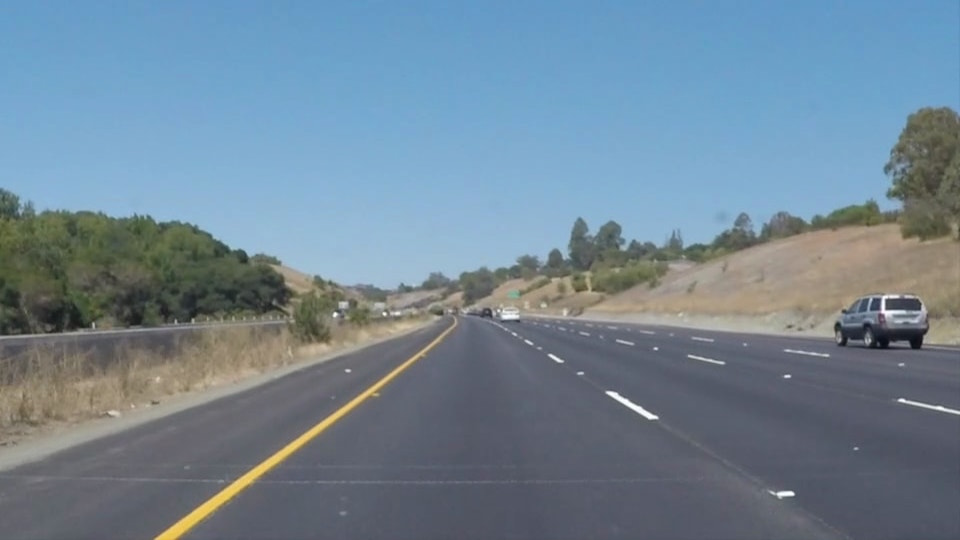
\includegraphics[scale=0.4]{lane_detection_steps/solidYellowCurve/0.jpg}
\caption{Example of image acquired by the camera.}
\label{fig:0}
\end{figure}
\subsection{Colour threshold}
The colour threshold consists of choosing a threshold value for each image channel (in our case the channels are red i.e., R, green, i.e., G or and blue, i.e., B). Each pixel having at least one channel value below the corresponding threshold is set to a black pixel ($(0, 0, 0)$). The resulting image is a high-contrast one.

The threshold value has been applied to all channels. For white lanes, a good value is $250$ but this does not work with yellow lines. Yellow being darker than white, the threshold has been lowered to $120$.

The result of this step is shown in \autoref{fig:1}.
\begin{figure}
\centering
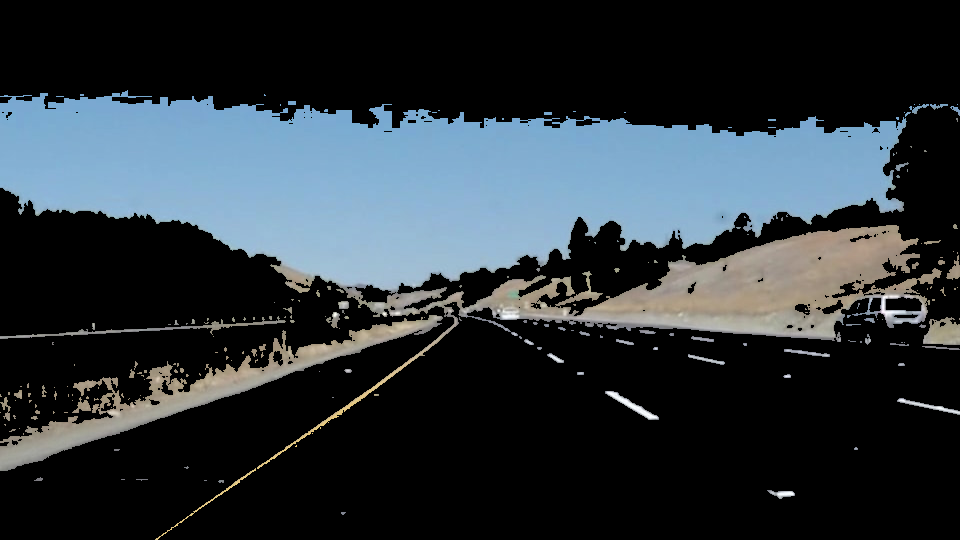
\includegraphics[scale=0.4]{lane_detection_steps/solidYellowCurve/1.jpg}
\caption{Image resulting from the colour thresholding step.}
\label{fig:1}
\end{figure}

\subsection{Gaussian filtering and Canny edge detection}
From the high-contrast image it becomes easier to identify edges using Canny filtering. However, Canny edge detection being a high pass filter that, as such, might amplify noise, it is considered good practice to apply a low pass filtering, in our case a Gaussian low pass filtering.

The result of this step is shown in \autoref{fig:2}.
\begin{figure}
\centering
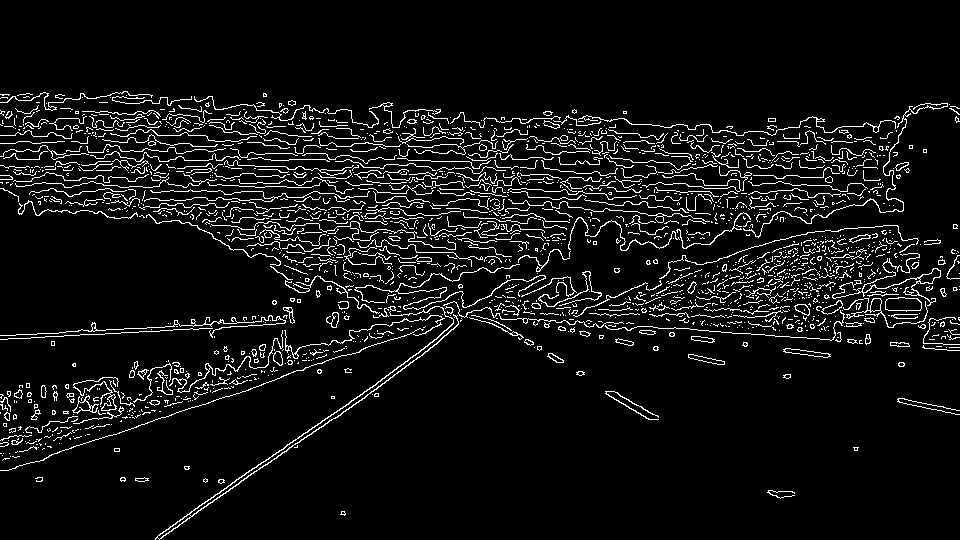
\includegraphics[scale=0.4]{lane_detection_steps/solidYellowCurve/2.jpg}
\caption{Image resulting from the Gaussian filtering and Canny edge detection steps.}
\label{fig:2}
\end{figure}

\subsection{Region selection}
The selected region is a trapezoid whose vertices are defined using the relative size of the image. Two vertices are at the bottom of the image, one to the left ($0.1$ of the image width) and one to the right ($0.9$ of the image width). The upper vertices are little below the median of the image ($0.6$ from the top of the image) and close to the half-width of the image ($0.45$ and $0.55$). The vertices and the image on which to apply region selection are passed to the function \cd+region_of_interest+ which sets first the pixel of the resulting image in the region of interest to $255$ and the rest to $0$ and then applies the a bitwise $OR$ operation.

The result of this step is shown in \autoref{fig:3}.
\begin{figure}
\centering
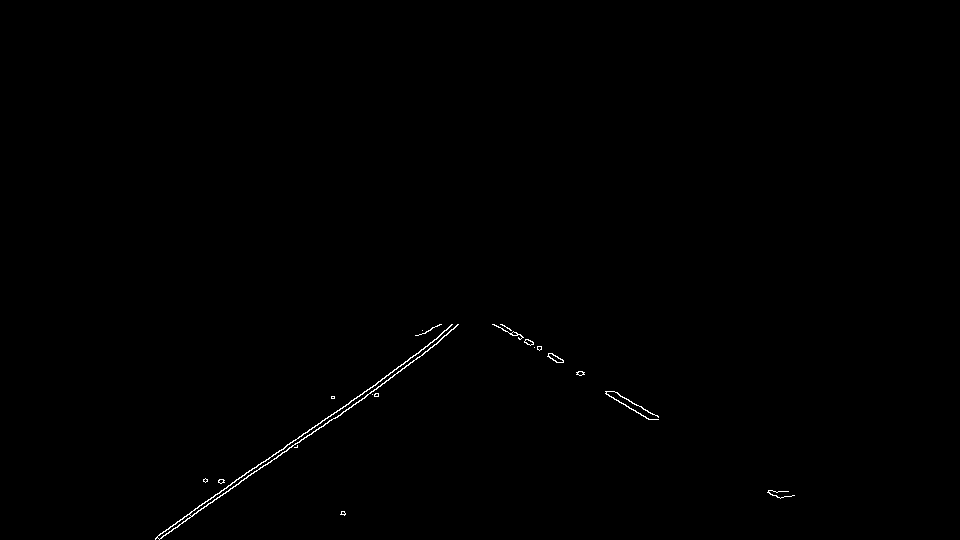
\includegraphics[scale=0.4]{lane_detection_steps/solidYellowCurve/3.jpg}
\caption{Image resulting from the region selection step.}
\label{fig:3}
\end{figure}

\subsection{Hough transforms}
Finally, hough transform is applied by calling the function \cd+hough_lines+. It is worth noting a big value of the parameter \cd+max_line_gap+ to make up for the non-solid lines.

The result of this step is shown in \autoref{fig:4}.

\begin{figure}
\centering
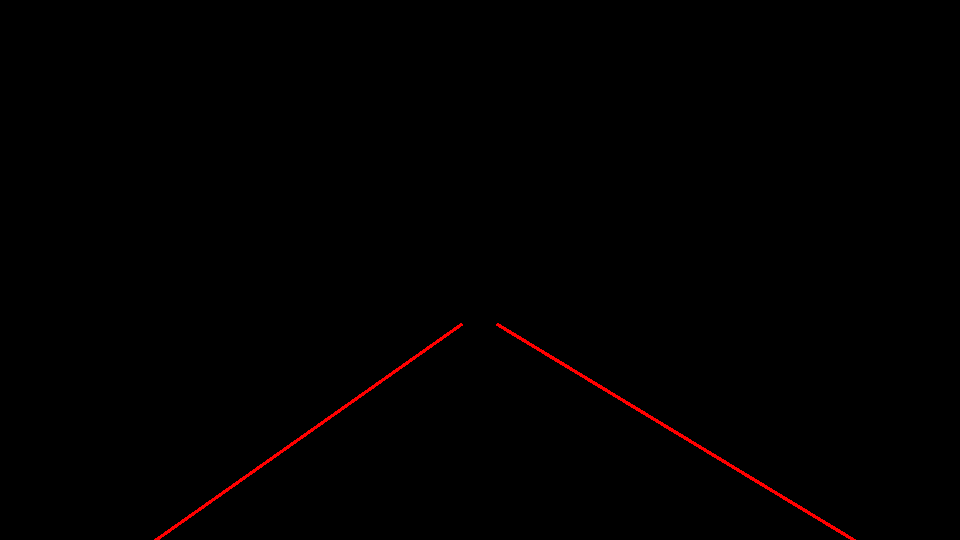
\includegraphics[scale=0.4]{lane_detection_steps/solidYellowCurve/4.jpg}
\caption{Image resulting from the Hough transform step.}
\label{fig:4}
\end{figure}

\subsection{Changes in the function draw\_lines}
The function \cd+draw_lines+ as it was before, for each lane line used to draw the many lines found (since lanes can thicker than one pixel) and when it is not solid, the resulted highlighted lane was shorter than its solid counterpart (see \autoref{fig:5}). To overcome this problem, \cd+draw_lines+ has been modified to produce only two lines resulting from two averages. To perform the averages among the same clusters, the slope has been considered: left lane lines have a negative slope whereas right lane lines have a positive slope. In this way the two averages can be carried out independently and two single lines are drawn.

However, some unexpected almost-horizontal lines used to appear in the images and videos from time to time. To weed those out, a further check has been added by considering the fact that the lane lines are almost vertical, hence the module of the slope is significantly big. For this reason lines with a slope module lower than a given threshold are not considered. This simple method works quite well (see \autoref{fig:6}).

\begin{figure}
\centering
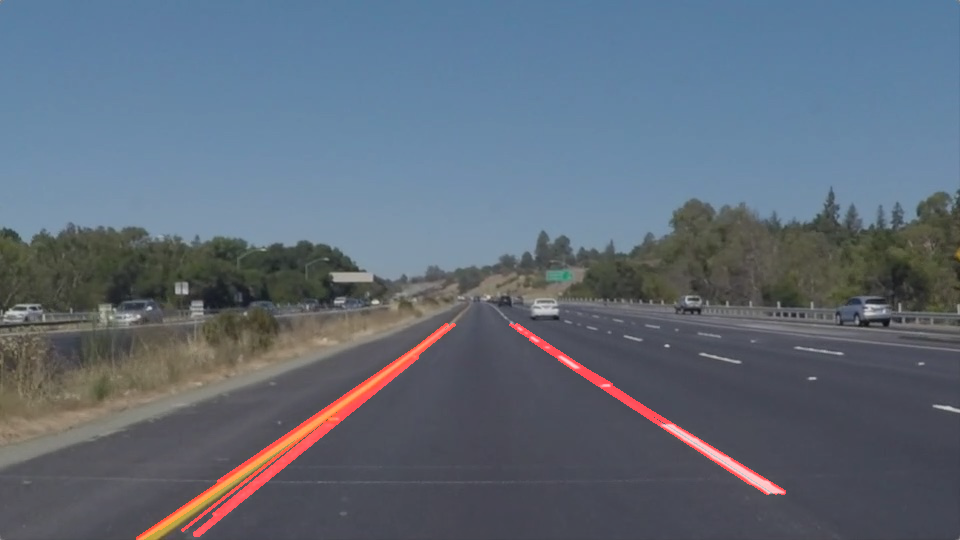
\includegraphics[scale=0.4]{test_images_output_raw/solidYellowLeft.jpg}
\caption{Image resulting from the original version \cd+draw_lines+ function.}
\label{fig:5}
\end{figure}

\begin{figure}
\centering
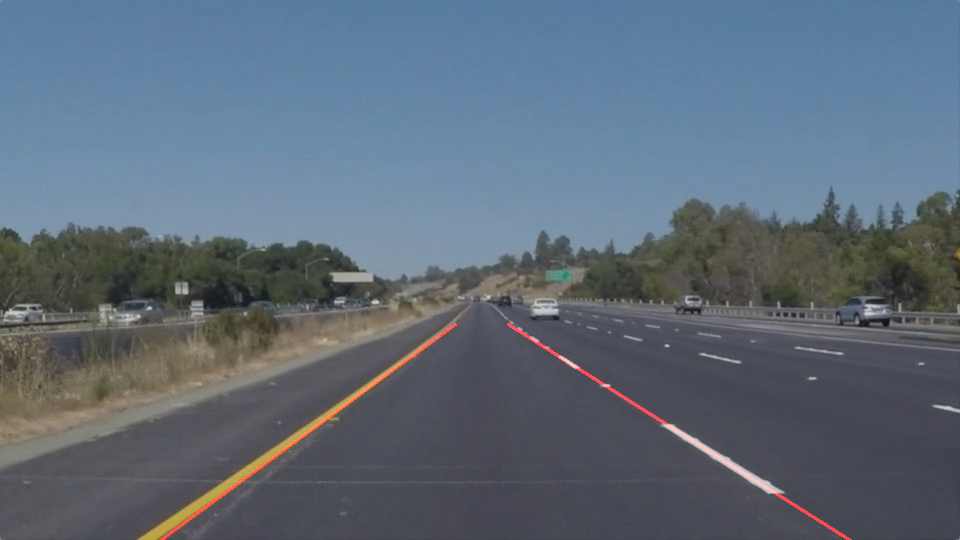
\includegraphics[scale=0.4]{test_images_output/solidYellowLeft.jpg}
\caption{Image resulting from the modified version of \cd+draw_lines+ function.}
\label{fig:6}
\end{figure}

\section{Possible shortcomings}
\subsection{Low visibility condition}
The algorithm is based on the assumption that lane lines in the images are much brighter than their background. In some cases this might not be the case. First of all, this might happen in condition of low-visibility: when light is not enough, the algorithm might not work and, even if it did, this would require the thresholds to be manually modified each time according to weather conditions. The same might happen if the lane lines are discoloured. Apart from the colour thresholds, also the Canny edge detector parameters should be modified accordingly.

\subsection{Road curves}
Another problem might be represented by road curves. In this case, when trying to fit lines to a curve, the algorithm becomes unstable and the resulting lines can be distorted.

\section{Possible improvements}
\subsection{Improvement in case of low visibility conditions}
Rather than choosing colour thresholds a-priori, it might be better to calculate a threshold for each image channel based on the some image analysis, for example, looking at he average pixel values of the full image or, even better, on the region of interest. In this way, one does not have to choose hyper-parameters for each weather condition.

\subsection{Improvements in case of road curve}
In case of road curves, line detection might be improved by fitting higher degree curves, but it might be difficult to combine this with the Hough transform. Another possible solution might be to fit a line for small areas of the region of interest, approximating in this way the curve with consecutive short lines.


\end{document}